\documentclass{article}

\usepackage[a4paper, total={6in, 8in}]{geometry}
\usepackage[utf8]{inputenc}
\usepackage{fancyhdr}
\usepackage{graphicx}
\usepackage{enumitem}

\pagestyle{fancy}
\fancyhf{}
\lhead{John J Li}
\rhead{CSE360 Summer 2021 Assignment 3}
\rfoot{\thepage}
\renewcommand{\headrulewidth}{0.4pt}

\setlength{\parskip}{1em}
\setlength\parindent{0px}
\title{CSE360 Summer 2021 Assignment 3}
\date{\today}
\author{John J Li}

\begin{document}
    \maketitle
    \thispagestyle{empty}
    \noindent\rule{\textwidth}{0.8pt}

    A client wants you to create a system for their vehicle rental service. Below is a list of vehicles
    they currently have:
    \begin{itemize}
        \item 
        Motorcycle
        \begin{itemize}
            \item 
            No doors
            \item
            Can carry between one to two passengers
            \item
            Two tires
        \end{itemize}
        \item 
        Sedan
        \begin{itemize}
            \item 
            Can have either two or four doors
            \item
            Can carry between two to five passengers
            \item
            Four tires
        \end{itemize}
        \item 
        Bus
        \begin{itemize}
            \item 
            One door
            \item
            Can carry up to sixty passengers
            \item
            Four tires
        \end{itemize}
    \end{itemize}

    %###################################################################################

    \section*{Problem 1}

    Below is a UML class diagram that models some of the vehicles described above. Fill in
    the missing “???” parts to make the diagram fully match the above description.

    \begin{center}
        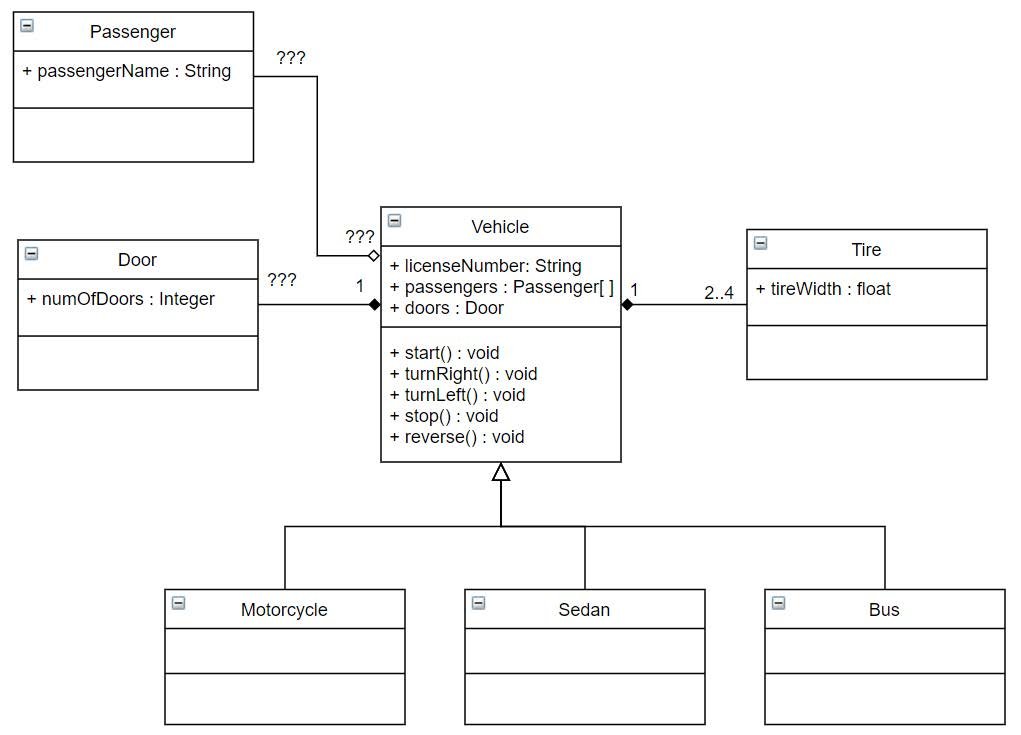
\includegraphics[scale=0.75]{Exercise 03_ Practice Problems.jpg}
    \end{center}

    \subsection*{Solution}

    \begin{center}
        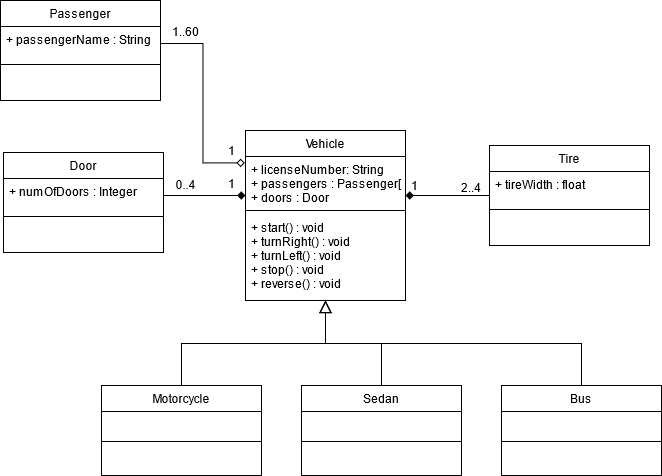
\includegraphics[scale=0.55]{E3_Q1.png}
    \end{center}

    %###################################################################################

    \section*{Problem 2}

    Passengers get on and off a bus frequently. Modify the UML class diagram from problem
    1 so that the “Bus” class has two methods:

    \begin{itemize}
        \item 
        passengerBoard()
        \begin{itemize}
            \item 
            The method is given an integer with the number of passengers getting
            onto the bus
        \end{itemize}
        \item
        passengerDisembark()
        \begin{itemize}
            \item 
            The method is given an integer with the number of passenger getting off
            the bus
        \end{itemize}
    \end{itemize}

    \subsection*{Solution}

    \begin{center}
        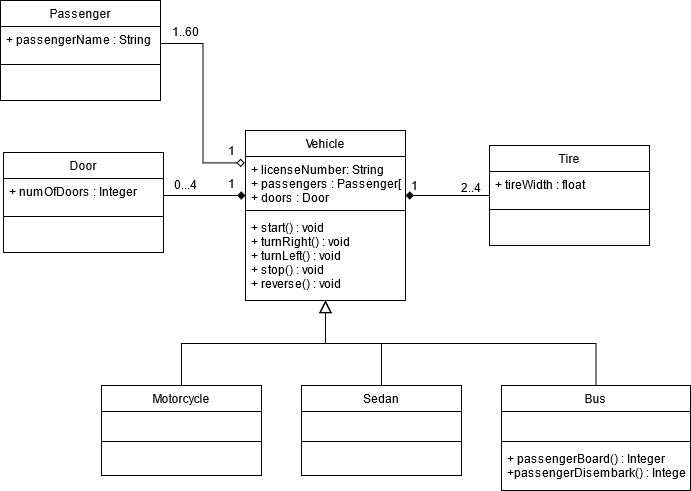
\includegraphics[scale=0.55]{E3_Q2.png}
    \end{center}

    %###################################################################################

    \section*{Problem 3}

    The client wants to search for a vehicle using the door type. Modify the UML 
    class diagram from problem 2 so that the “Door” class
    has an attribute called “doorType” of type “String”.

    \subsection*{Solution}

    \begin{center}
        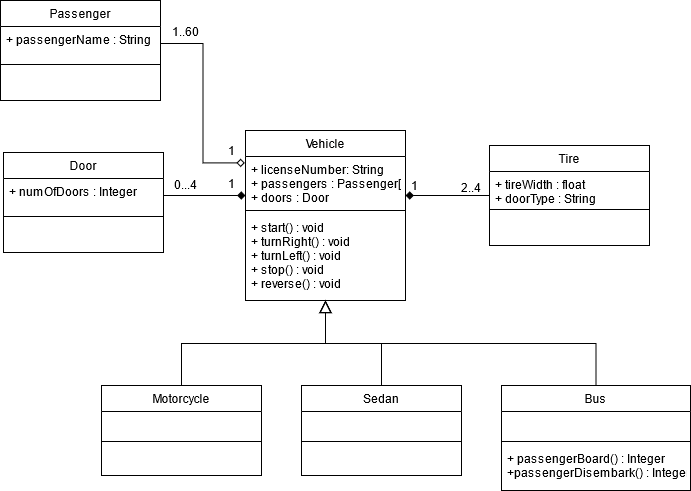
\includegraphics[scale=0.55]{E3_Q3.png}
    \end{center}

    %###################################################################################

    \section*{Problem 4}

    The client has started to incorporate semi-trucks into their business. These vehicles
    typically have:
    \begin{itemize}
        \item 
        Two doors
        \item
        Can carry up to two passengers
        \item
        Can have between six to ten tires
    \end{itemize}
    Modify the UML class diagram from problem 3 to include this new vehicle type in the
    model.

    \subsection*{Solution}

    \begin{center}
        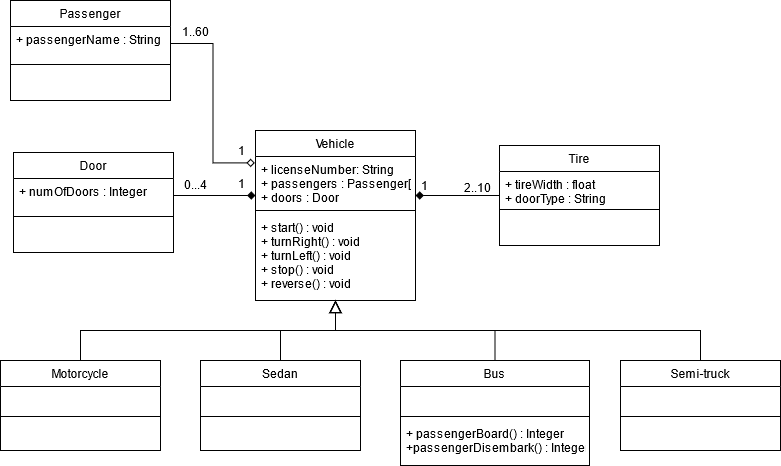
\includegraphics[scale=0.55]{E3_Q4.png}
    \end{center}

\end{document}